% Datasets

\chapter{Jeu de données} % Main chapter title

\label{Datasets} % For referencing the chapter elsewhere, use \ref{Datasets} 

%----------------------------------------------------------------------------------------

\section{Provenance des données utilisées}
\label{sec:dataset_origin}

Les données avec lesquelles nous travaillons correspondent aux mesures réalisées par le calorimètre. Comme illustré sur la figure \ref{fig:cern_calorimeter}, celui-ci forme un cylindre au centre duquel se produisent les collisions de particules.

\begin{figure}[hbt!]
    \centering
    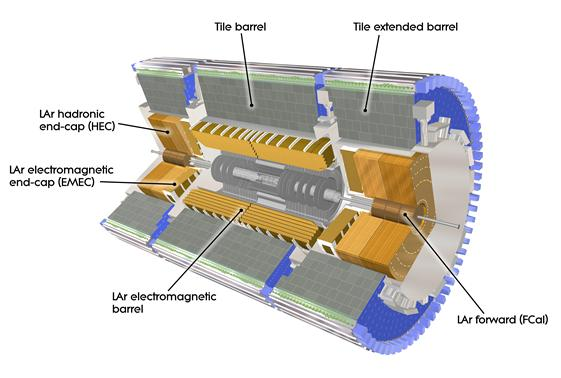
\includegraphics[scale=0.4]{Figures/dataset/cern_calorimeter.jpg}
    \caption{Représentation du calorimètre de l'expérience \acrshort{atlas} \cite{noauthor_computer_nodate}.}
    \label{fig:cern_calorimeter}
\end{figure}

Le détecteur est composé de plusieurs couches, comme visible sur la figure \ref{fig:calorimeter_structure}, qui possèdent chacune sa propre résolution. Les données issues de ces capteurs sont par la suite déroulées afin d'être représentées sur un plan à deux dimensions. C'est pourquoi nous retrouvons sur l'axe $\phi$ les valeurs allant de $-3.14$ à $3.14$ correspondant à $2\pi$ soit la circonférence du cylindre. Cela implique que les cellules aux coordonnées $\phi$ $-3.14$ et $3.14$ sont censées être plus proches entre elles que de la coordonnée $0$, de par le fait qu'elles sont issues d'un cylindre. Dans notre utilisation des données, afin de ne pas complexifier l'apprentissage de nos modèles pour la détection, nous ne prendrons pas en compte les jets présents dans ces extrémités.

\begin{figure}[hbt!]
    \centering
    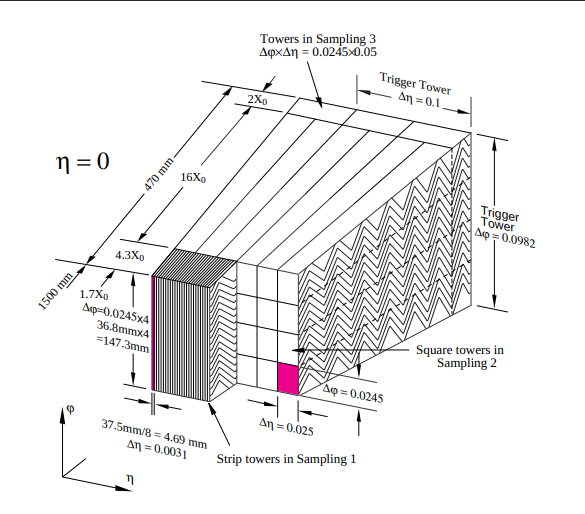
\includegraphics[scale=0.4]{Figures/dataset/structure_of_the_calorimeter.png}
    \caption{Structure du calorimètre de l'expérience \acrshort{atlas} \cite{noauthor_atlas_1996} (Figure 1-2).}
    \label{fig:calorimeter_structure}
\end{figure}

\break

En plus des données captées par des expériences réelles, le \acrshort{cern} possède un outil leur permettant de générer des simulations et d'indiquer les paramètres de leur choix. Ainsi, les données utilisées dans notre travail sont issues de ces simulations et nous ont été fournies directement par Claire Antel, post-doctorante à l'Université de Genève travaillant également sur le projet \acrshort{atlas} au \acrshort{cern}. Parmi celles-ci, le rayon des jets nous a été communiqué comme ayant été défini à $0.4$, et deux jeux de données nous ont été mis à disposition. Le premier contient un phénomène nommé "PileUp", tandis que le deuxième en est dépourvu.

Le "PileUp" apparaît lorsque plusieurs collisions de particules se produisent en même temps ou presque au sein du détecteur aux côtés de l'interaction d'intérêt. Les données obtenues lors d'une interaction d'intérêt peuvent alors être superposées aux valeurs liées à d'autres collisions. Les données "PileUp" sont plus proches de ce qu'une expérience réelle pourrait produire, mais ajoutent la complexité liée à la gestion du "PileUp".

Afin d'évaluer les performances pures des modèles utilisés face à la détection de jets, nous avons décidé d'utiliser les données ne contenant pas de "PileUp" dans notre travail.\\

Le jeu de données retenu est donc composé de vingt fichiers .h5. Ceux-ci sont divisés en deux catégories :

Dix d'entre eux contiennent les informations liées aux détections du calorimètre pour chaque expérience, comme ; les coordonnées $\eta \times \phi$, l'énergie, ou encore l'impulsion transverse des cellules.

Les dix autres sont liés aux fichiers précédents, et contiennent les informations relatives aux jets détectés dans chaque expérience, comme les coordonnées $\eta \times \phi$ de l'emplacement du jet.

Le premier ensemble nous permet de générer les images que nous passons à nos modèles, tandis que le deuxième nous sert à générer les labels à l'aide des coordonnées $\eta \times \phi$ des jets présents dans chaque expérience.

\section{Structure des fichiers}
\label{sec:files_structure}

Comme expliqué dans la section précédente \ref{sec:dataset_origin}, les données sont décomposées dans deux fichiers .h5 et retracent un total de mille expériences. Le premier contient toutes les informations relatives à la détection effectuées par le calorimètre. Et le second comporte les données liées aux jets détectés.

Dans le fichier des données du calorimètre, celui-ci possède l'objet nommé "caloCells" dans lequel nous retrouvons deux autres objets "1d" et "2d". Le premier inclut les éléments relatifs aux événements, tandis que le deuxième contient les données. C'est ce dernier qui nous intéresse. Nous allons parcourir les mille événements contenus dans l'objet "2d", qui possèdent une multitude d'informations, cependant dans le cadre de notre travail nous utiliserons uniquement les tableaux : $cell\_E$, l'énergie; $cell\_Sigma$, le niveau de bruit; $cell\_eta$, la coordonnée eta; $cell\_phi$, la coordonnée phi; et $cell\_pt$, l'impulsion transverse, qui contiennent les valeurs de chaque cellules.

Le fichier des informations des jets, possède la même structure initiale, avec d'autres tableaux contenant les valeurs des différents jets. Ces tableaux doivent tous posséder la même taille, or comme le nombre de jets peut varier d'une expérience à une autre, les tableaux sont définis à une taille fixe de trente. Le nombre de jets au sein des fichiers n'est jamais équivalent ou même proche de ce nombre comme nous pouvons le voir sur la figure \ref{fig:jet_distribution} . Concernant les variables utilisées, nous avons besoin des tableaux : $AntiKt4EMTopoJets\_eta$, la coordonnée $\eta$; et $AntiKt4EMTopoJets\_phi$ la coordonnée $\phi$, qui contiennent soit les coordonnées des jets de l'expérience courante, soit la valeur $nan$ pour compléter le tableau.

\begin{figure}[hbt!]
    \centering
    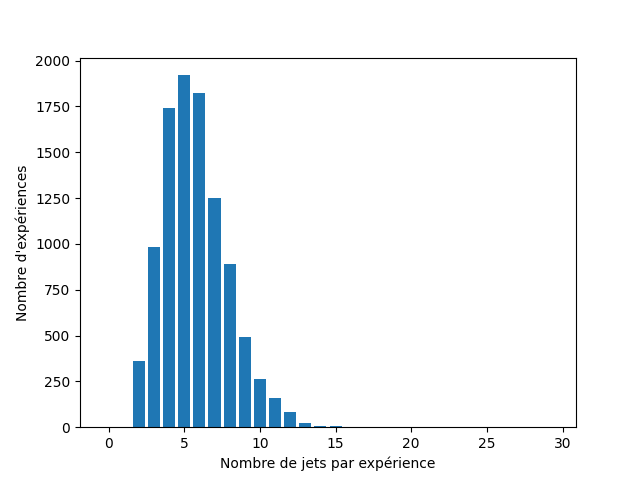
\includegraphics[scale=0.7]{Figures/dataset/file_jet_distribution.png}
    \caption{Distribution du nombre de jets par expérience à partir des fichiers de données utilisés}
    \label{fig:jet_distribution}
\end{figure}

Il reste évidemment beaucoup d'informations à disposition dans ces fichiers, néanmoins, dans notre cadre, nous nous contentons d'utiliser celles que nous avons indiquées.

\section{Prise en main des données issues du calorimètre}

Avant de pouvoir générer des images et des labels pour nos modèles, il nous a d'abord fallu prendre en main les données, les comprendre, les nettoyer, et les manipuler afin d'en extraire l'essence.

Pour cela, nous avons tout d'abord débuté en affichant sur un plan à deux dimensions les emplacements des capteurs comme visible sur la figure \ref{fig:calocells_location}. Nous voyons que l'emplacement des capteurs n'est pas régulier sur l'ensemble du calorimètre, et qu'il pourrait être par conséquent plus complexe de réaliser des détections de jets dans les zones moins fournies en capteurs. En revanche, nous constatons que la région dans l'intervalle $\eta \in \mathbb{R} : \eta \in [-2.4;2.4]$ et $\phi \in \mathbb{R} : \phi \in [-3.14;3.14]$ possède des capteurs disposés plus régulièrement.

\begin{figure}[hbt!]
    \centering
    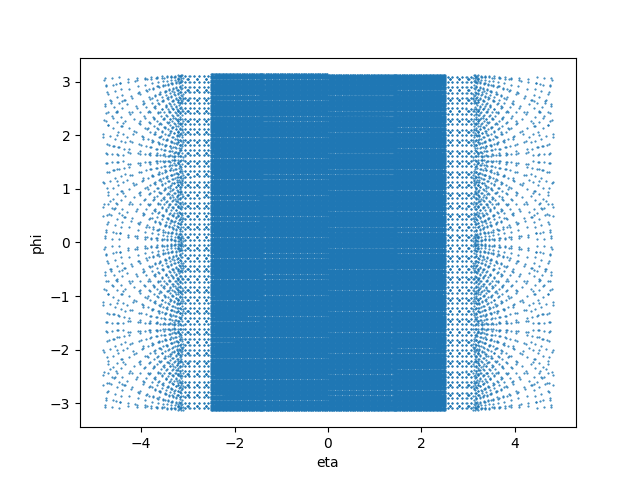
\includegraphics[scale=0.7]{Figures/dataset/calorimeter_cells.png}
    \caption{Emplacement des cellules du calorimètre}
    \label{fig:calocells_location}
\end{figure}

En nous concentrant sur l'intervalle défini, nous pouvons voir sur la figure \ref{fig:calocells_location_eta_reduced} que deux zones verticales symétriques moins denses en capteurs apparaissent vers $\eta$ $-1.45$ et $1.45$. Cela n'est pas critique, mais il est bon de noter que plus tard, lors de la création d'une matrice à partir des données du calorimètre, des artéfacts peuvent en résulter. Ces derniers sont des anomalies non souhaitées et qui ne sont pas représentatives de ce que nous souhaitons étudier. Dans notre cas, ils peuvent apparaître de par la disposition des capteurs, et venir complexifier voire fausser les résultats de nos modèles en leur faisant apprendre des caractéristiques non pertinentes.

\begin{figure}[hbt!]
    \centering
    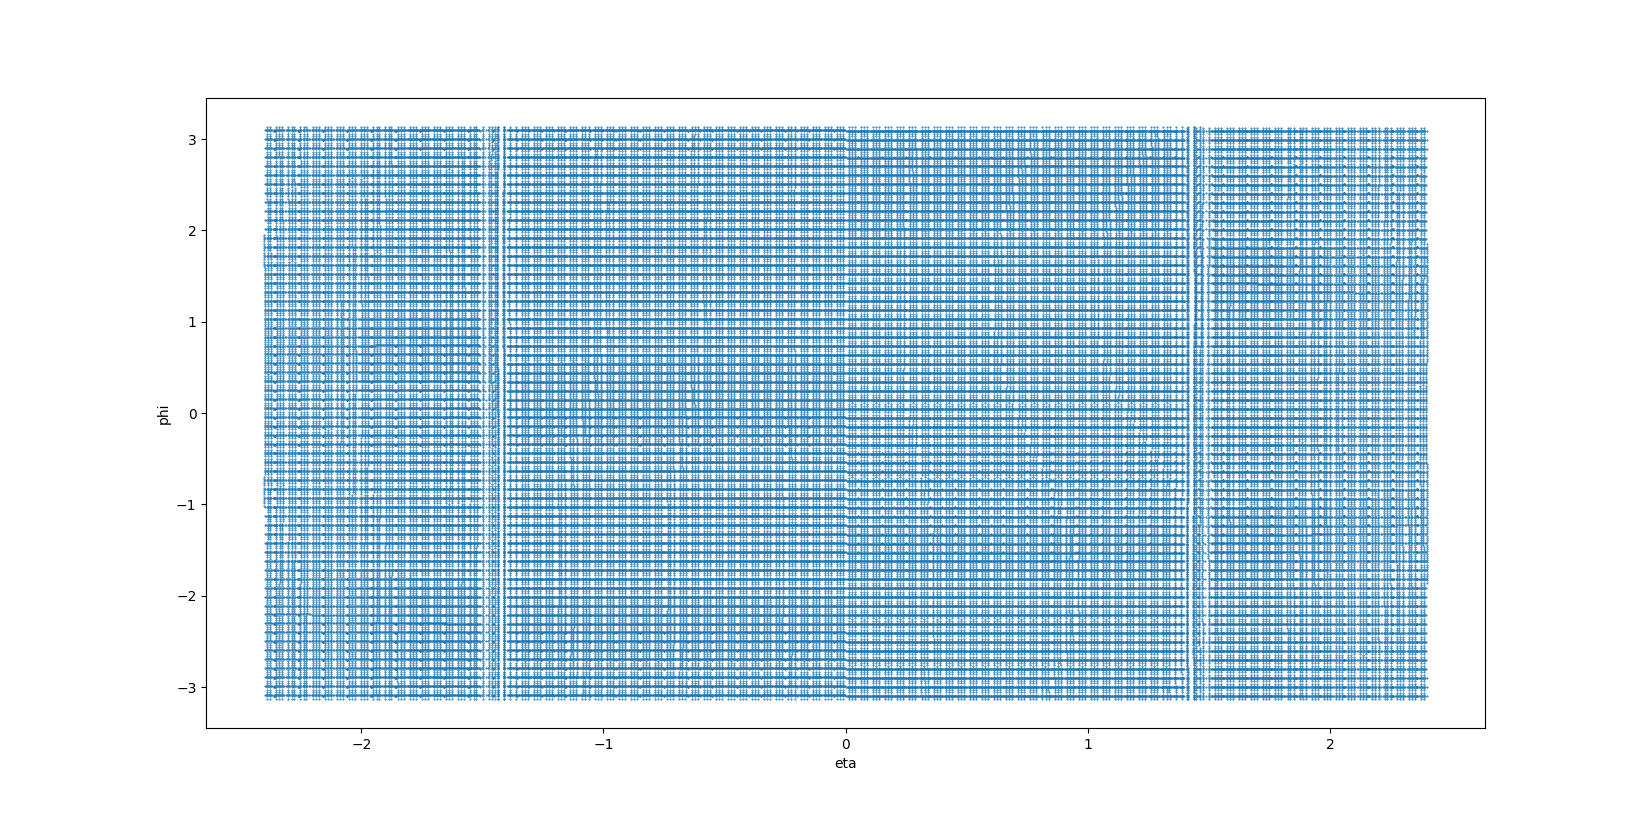
\includegraphics[scale=0.3]{Figures/dataset/calorimeter_cells_eta_reduced.png}
    \caption{Emplacement des cellules du calorimètre dans l'intervalle $\eta \in \mathbb{R} : \eta \in [-2.4;2.4]$ et $\phi \in \mathbb{R} : \phi \in [-3.14;3.14]$}
    \label{fig:calocells_location_eta_reduced}
\end{figure}

\break

En agrandissant la région dense en capteurs autour de $0$, nous voyons comment ceux-ci sont répartis grâce à la figure \ref{fig:calocells_location_eta_reduced_zoomed_in}. Nous constatons qu'ils ne sont pas tous disposés à distance égale les un des autres, étant donné qu'ils correspondent aux différentes couches de capteurs possédant une granularité différente. Il est important de prendre en compte cette répartition, car cela peut être une source d'artéfacts sur l'image générée à partir des données.

\begin{figure}[hbt!]
    \centering
    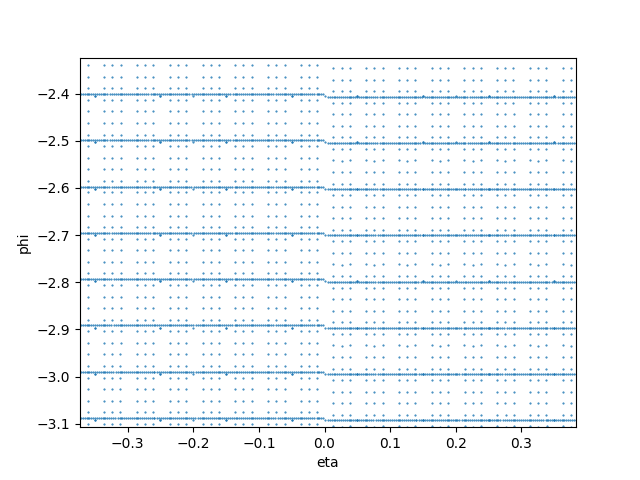
\includegraphics[scale=0.7]{Figures/dataset/calo_cells_zoomed_in.png}
    \caption{Emplacement des cellules du calorimètre zoomé}
    \label{fig:calocells_location_eta_reduced_zoomed_in}
\end{figure}

\break

\section{Manipulation et préparation des données issues du calorimètre}

\subsection{Création d'une matrice}

L'étape suivant la visualisation de l'emplacement des capteurs du calorimètre consiste à réaliser une matrice pour représenter celle-ci. Pour ce faire, nous avons besoin de connaître la distance entre deux capteurs. Après une discussion avec la professeure Anna Sfyrla de l'Université de Genève travaillant également au \acrshort{cern} sur le projet \acrshort{atlas}, il en est ressorti d'utiliser une distance de $0.025$ pour $\eta$ et $\phi$ correspondant au "Sampling 2" du calorimètre \cite{noauthor_atlas_1996}.

À partir de cette information nous pouvons donc construire une matrice utilisant un pas de $0.025$ sur l'intervalle $\eta \in \mathbb{R} : \eta \in [-2.4;2.4]$ et $\phi \in \mathbb{R} : \phi \in [-3.14;3.14]$. La taille de celle-ci est de $\eta \times \phi = 193 \times 253$. Afin de pouvoir y insérer des valeurs, nous commençons par arrondir les coordonnées $\eta \times \phi$ à 0.025, puis à l'aide des transformations suivantes :

\label{formula:compute_indices}

\[Indice \: \eta \: Cell_{i} = (Cell_{i_{\eta}} + 2.4) / (2.4*2) \cdot (W-1)\]
\[Indice \: \phi \: Cell_{i} = (Cell_{i_{\phi}} + 3.15) / (3.15*2) \cdot (H-1)\]

où $W$ et $H$ correspondent respectivement à la taille de la matrice pour $\eta$ et $\phi$. Nous calculons les indices $\eta \times \phi$ pour notre matrice de la cellule $i$ à partir des coordonnées arrondies. Notons que nous utilisons pour $\phi$ la valeur de $3.15$ que nous avons obtenu en arrondissant $\pi$ vers le haut.

Nous pouvons à présent ajouter à chaque indice de notre matrice l'énergie de chaque cellule. Étant donné que nous avons réalisé un arrondi sur les coordonnées, nous allons additionner les valeurs dans un même indice afin de ne pas perdre d'énergie lors de la transformation.\\

\subsection{Normalisation de l'énergie avec le niveau de bruit et filtrage des données}

L'énergie en provenance du calorimètre contient également le bruit de la cellule en question. Afin de normaliser les valeurs de celles-ci, nous divisons l'énergie par le niveau de bruit pour en faire ressortir le signal. Cette méthode nous permet d'obtenir un ratio utile pour comparer les cellules, mais surtout de distinguer les signaux pertinents du bruit de fond.

Si nous observons à quoi ressemble une de nos matrices actuellement, nous obtenons un résultat similaire à celui de la figure \ref{fig:matrix_post_energy_over_noise_no_filter}. Nous y voyons quelques pixels ressortir, ainsi qu'une échelle d'énergie sur bruit très élevée. Bien que cela soit un début, nous faisons face à deux problèmes; les cellules contenant peu d'énergie sur bruit ne sont pas visibles, et entre deux expériences cette valeur peut énormément varier.

\begin{figure}[hbt!]
    \centering
    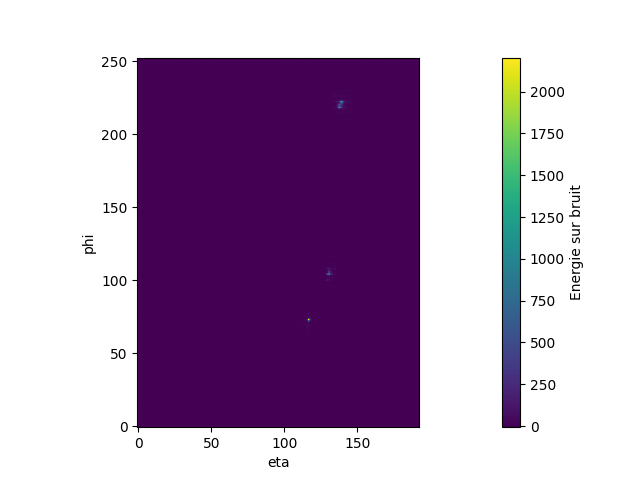
\includegraphics[scale=0.7]{Figures/dataset/matrix_post_energy_over_noise_no_filter.png}
    \caption{Matrice générée à partir de l'énergie sur bruit des cellules du calorimètre pour l'expérience 0 du fichier : \url{user.cantel.33075755.\_000001.calocellD3PD\_mc16\_JZW4.r14423}.}
    \label{fig:matrix_post_energy_over_noise_no_filter}
\end{figure}

\break

La distribution de l'énergie sur bruit supérieure à $0$ de chaque cellule de toutes les expériences du fichier $user.cantel.33075755.\_000001.calocellD3PD\_mc16\_JZW4.r14423$ visible sur la figure \ref{fig:hist_energy_over_sigma}, nous montre que la majorité d'entre elles possèdent une énergie sur bruit relativement faible. Ainsi, même si les cellules avec une valeur très élevée sont intéressantes, il ne faut pas pour autant négliger celles dont l'énergie sur bruit est plus modeste.

\begin{figure}[hbt!]
    \centering
    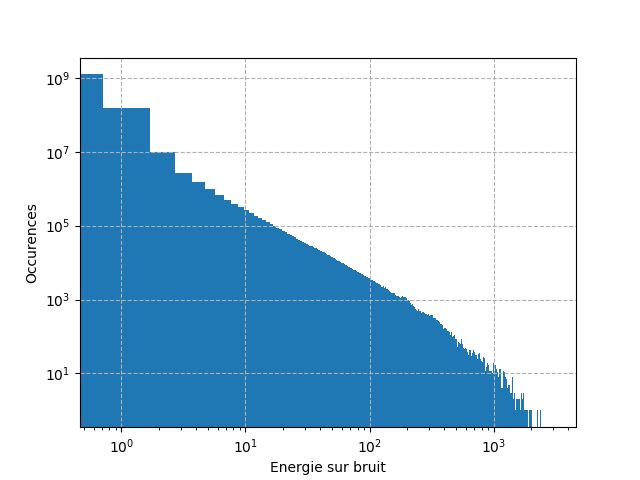
\includegraphics[scale=0.7]{Figures/dataset/hist_energy_over_sigma.png}
    \caption{Histogramme de l'énergie sur bruit supérieure à 0 de toutes les cellules parmis toutes les expériences du fichier : \url{user.cantel.33075755.\_000001.calocellD3PD\_mc16\_JZW4.r14423}.}
    \label{fig:hist_energy_over_sigma}
\end{figure}

\break

Pour limiter la quantité d'énergie sur bruit maximum qu'une cellule peut atteindre dans le but de rendre les autres valeurs plus visibles, mais également afin d'éliminer les faibles valeurs pouvant être confondues avec du bruit, nous définissons deux seuils.

Le premier va retirer les cellules dont l'énergie sur bruit est inférieure à une valeur donnée. Tandis que le second fixe une valeur maximum qui est attribuée à toutes celles la dépassant. Cela a pour but d'éviter que des cellules très énergétiques en "cachent" d'autres sur notre matrice.

Les valeurs définies pour les seuils nous ont été indiquées par la Professeure Anna Sfyrla. Nous utilisons exclusivement les valeurs pour lesquelles l'énergie sur bruit est supérieure à $2$ (qui est également celle recommandée par le CERN \cite{gross_frequentist_2011}). Quant à la valeur maximum qui peut être attribuée à une cellule, celle-ci est définie à $6$, légèrement au-dessus du traditionnel seuil de $5$ \cite{lyons_discovering_2013}.\\

Visualisons à présent notre matrice représentée à la figure \ref{fig:matrix_post_energy_over_noise} construite en utilisant nos seuils, et sur laquelle des cercles rouges correspondent à l'emplacement des jets. Même si cela n'est pas très visible, nous voyons quelques cellules en plus, et surtout une échelle d'énergie sur bruit bien plus petite que sur la figure \ref{fig:matrix_post_energy_over_noise_no_filter}. Cependant, nous n'avons toujours pas résolu nos deux problèmes précédents. En effet, même si la valeur maximum d'une cellule est fixée à $6$, sur notre matrice nous additionnons les valeurs des cellules correspondant aux mêmes indices. Cette façon de faire implique que certains indices peuvent posséder des valeurs encore trop élevées cachant ainsi ceux à l'énergie sur bruit plus faible.

\begin{figure}[hbt!]
    \centering
    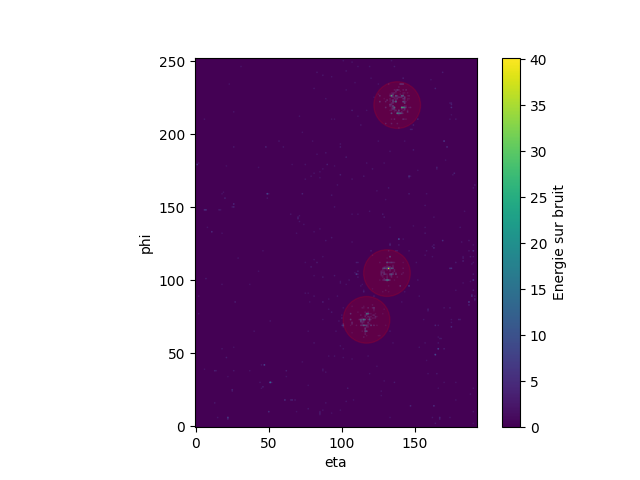
\includegraphics[scale=0.7]{Figures/dataset/matrix_post_energy_over_noise.png}
    \caption{Matrice générée à partir de l'énergie sur bruit filtrée des cellules du calorimètre supérieure à 2 pour l'expérience 0 du fichier : \url{user.cantel.33075755.\_000001.calocellD3PD\_mc16\_JZW4.r14423}.}
    \label{fig:matrix_post_energy_over_noise}
\end{figure}

\break

\subsection{Normalisation des matrices entre 0 et 1}

Afin de remédier à ces problèmes, nous normalisons nos valeurs pour qu'elles soient contenues entre $0$ et $1$. Pour cela, nous souhaitons utiliser une fonction non linéaire qui va accentuer le rôle des cellules avec des valeurs plus faibles, tout en réduisant l'impact des valeurs très élevées. Étant donné que grâce à nos seuils nos valeurs sont toujours positives, une fonction parfaite pour ce rôle serait le logarithme. Néanmoins, en gardant en tête que nous souhaitons implémenter tout cela sur \acrshort{fpga}, la fonction logarithmique étant très coûteuse, nous allons utiliser une alternative. La fonction retenue est :

\[f(x) = 1-\frac{(\mu+\sigma)}{((\mu+\sigma)+x)}\]

où $\mu$ et $\sigma$ correspondent respectivement à la moyenne et à l'écart-type des énergies sur bruit de toutes les cellules. Comme nous pouvons le voir sur la figure \ref{fig:personalized_function}, celle-ci nous assure que nos valeurs positives le restent, tout en donnant de l'importance aux faibles valeurs, et en diminuant l'impact des grandes. Par ailleurs, en utilisant la moyenne et l'écart-type de l'expérience en cours, cela nous permet d'adapter notre fonction pour que son comportement s'adapte aux valeurs rencontrées.

\begin{figure}[hbt!]
    \centering
    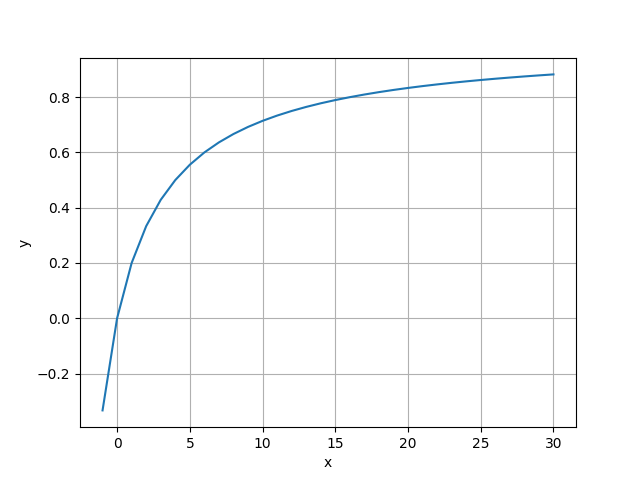
\includegraphics[scale=0.7]{Figures/dataset/personalized_function.png}
    \caption{Visualisation de la fonction utilisée pour normaliser les valeurs d'énergie sur bruit : $f(x) = 1-(\mu+\sigma)/((\mu+\sigma)+x)$ où $\mu$ est défini à $5$ et $\sigma$ à 1.}
    \label{fig:personalized_function}
\end{figure}

L'application de notre fonction sur notre matrice de la figure \ref{fig:matrix_post_energy_over_noise} nous donne le résultat affiché sur la figure \ref{fig:matrix_post_energy_over_noise_normalized}. Nous voyons à présent sur celle-ci que les zones contenant des jets ressortent beaucoup mieux et sont plus facilement identifiables. Par ailleurs, nous constatons aussi que d'autres cellules contenant de l'énergie sur bruit de façon beaucoup moins intense deviennent visibles.

L'utilisation de notre fonction nous démontre ses biens faits, et la place importante qu'elle occupe dans la préparation des données.

\begin{figure}[hbt!]
    \centering
    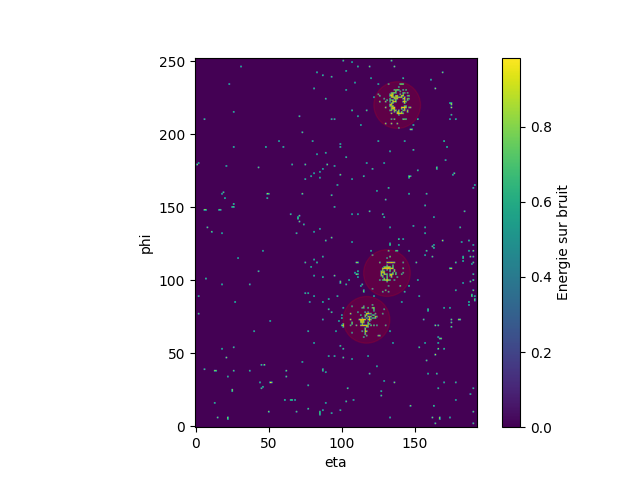
\includegraphics[scale=0.7]{Figures/dataset/matrix_post_energy_over_noise_normalized.png}
    \caption{Matrice générée à partir de l'énergie sur bruit des cellules du calorimètre supérieure à 2 puis normalisée pour l'expérience 0 du fichier : \url{user.cantel.33075755.\_000001.calocellD3PD\_mc16\_JZW4.r14423}.}
    \label{fig:matrix_post_energy_over_noise_normalized}
\end{figure}

\break

\subsection{Utilisation de canaux}

Bien que notre préparation des données semble faire correspondre les jets aux zones où des groupes de cellules possèdent une énergie sur bruit plus élevé, nous remarquons sur la figure \ref{fig:matrix_post_energy_over_noise_normalized_not_all_jets_visible} que certains d'entre eux, bien qu'indiqués présents, ne semblent pas ressortir. C'est le cas notamment pour le jet défini environ aux coordonnées $\eta \times \phi = 139 \times 220$. Celui-ci possède quelques cellules avec des valeurs autour de $0.8$ mais cela n'est pas fondamentalement différent d'autres zones de notre matrice qui ne contiennent pas de jets.

Ainsi, l'énergie sur bruit ne semble pas suffisante à elle seule afin de réaliser la détection de jets. Dans l'article traitant de l'algorithme $anti-k_t$ \cite{cacciari_anti-k_t_2008} réalisant des regroupements de ces derniers, l'impulsion transverse que nous possédons dans notre jeu de données est utilisée.

Sur la figure \ref{fig:matrix_post_energy_over_noise_normalized_not_all_jets_visible_e_o_n_and_pt}, nous pouvons observer la zone du jet vue par les deux matrices issues de l'énergie sur bruit à gauche, et de l'impulsion transverse à droite. Bien qu'il s'agisse des mêmes cellules concernées, nous pouvons voir que les valeurs de celles-ci sont différentes.

Utiliser les deux matrices ainsi générées pourrait être bénéfique pour l'apprentissage et la détection de jets par nos modèles.

Nous créons donc une matrice contenant trois canaux afin de pouvoir l'utiliser comme une image. Le premier canal contient les valeurs de l'énergie sur bruit normalisées. Le deuxième est constitué de l'impulsion transverse normalisée. Et finalement, le troisième est un canal vide rempli par des zéros. Cette dernière pourrait potentiellement accueillir d'autres valeurs pertinentes pour la détection de jets. 

\begin{figure}[hbt!]
    \centering
    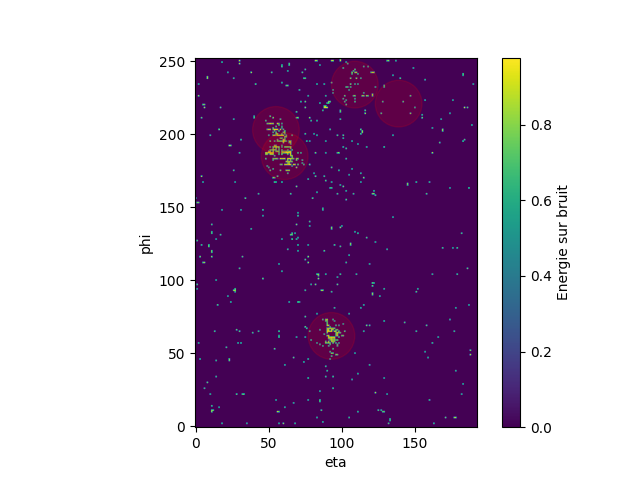
\includegraphics[scale=0.7]{Figures/dataset/matrix_post_energy_over_noise_normalized_not_all_jets_visible.png}
    \caption{Matrice générée à partir de l'énergie sur bruit des cellules du calorimètre supérieure à 2 puis normalisée pour l'expérience 9 du fichier : \url{user.cantel.33075755.\_000001.calocellD3PD\_mc16\_JZW4.r14423}.}
    \label{fig:matrix_post_energy_over_noise_normalized_not_all_jets_visible}
\end{figure}

\begin{figure}[hbt!]
    \centering
    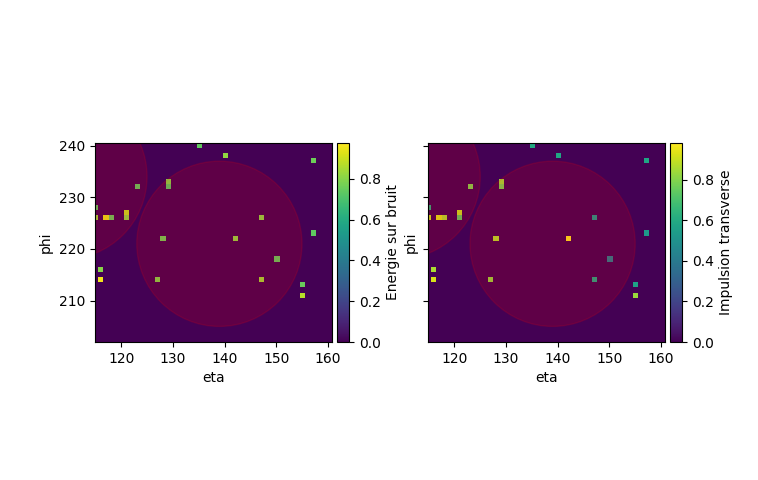
\includegraphics[scale=0.7]{Figures/dataset/matrix_post_energy_over_noise_normalized_not_all_jets_visible_e_o_n_and_pt.png}
    \caption{Matrices générées à partir de l'énergie sur bruit (à gauche) et de l'impulsion transverse (à droite) des cellules du calorimètre supérieure à $2$ puis normalisées pour l'expérience 9 du fichier : \url{user.cantel.33075755.\_000001.calocellD3PD\_mc16\_JZW4.r14423}.}
    \label{fig:matrix_post_energy_over_noise_normalized_not_all_jets_visible_e_o_n_and_pt}
\end{figure}

\break

\subsection{Gestion des artéfacts}

Même s'ils ne sont pas clairement visibles, les images générées jusqu'à présent contiennent des artéfacts. Ceux-ci deviennent visibles lorsque nous diminuons le seuil des valeurs acceptées dans notre matrice. En le passant de $2$ à $0$, nous obtenons le résultat de la figure \ref{fig:matrix_post_traitement_artefacts}. Grâce à la normalisation, précédemment appliquée, nous pouvons y voir apparaître des lignes verticales symétriques, ainsi que des lignes horizontales régulières qui ne sont pas sans nous rappeler la disposition des capteurs du calorimètre.

\begin{figure}[hbt!]
    \centering
    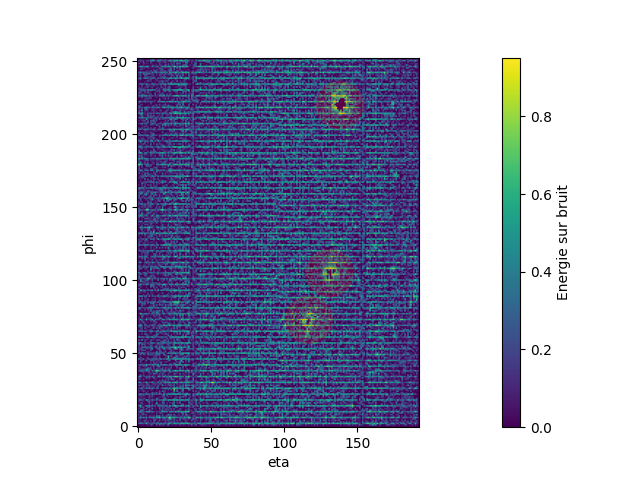
\includegraphics[scale=0.7]{Figures/dataset/matrix_post_traitement_artefacts.png}
    \caption{Matrice générée à partir de l'énergie sur bruit des cellules du calorimètre supérieure à 0 puis normalisée pour l'expérience 0 du fichier : \url{user.cantel.33075755.\_000001.calocellD3PD\_mc16\_JZW4.r14423}.}
    \label{fig:matrix_post_traitement_artefacts}
\end{figure}

\break

Une approche qui nous a été conseillée par Leon Bozianu, doctorant à l'Université de Genève dans l'équipe de la professeure Anna Sfyrla, était d'utiliser une distance entre les capteurs égale à $\delta \eta \times \delta \phi = 0.1 \times 0.1$ correspondant à la plus grande granularité des capteurs.

En diminuant la granularité de notre matrice, mais en conservant l'énergie sur bruit des cellules supérieures à $0$, nous obtenons des matrices comme celle de la figure \ref{fig:matrix_post_traitement_reduced_0} d'une taille de $\eta \times \phi = 49 \times 64$. Certains artéfacts sont toujours présents, mais de façon plus nuancée.

\begin{figure}[hbt!]
    \centering
    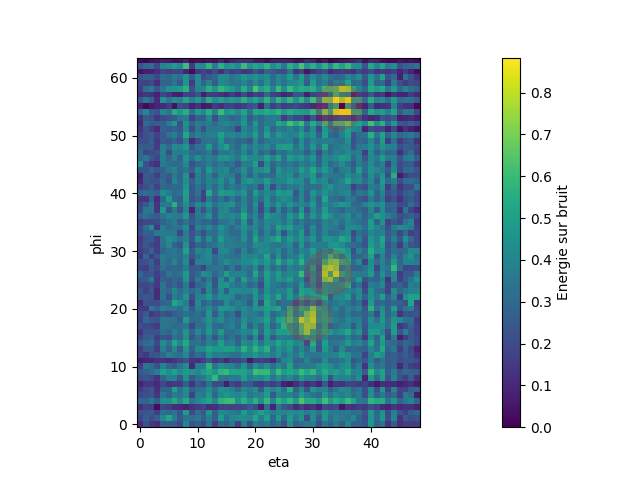
\includegraphics[scale=0.7]{Figures/dataset/matrix_post_traitement_reduced_0.png}
    \caption{Matrice d'un pas de $0.1 \times 0.1$ générée à partir de l'énergie sur bruit des cellules du calorimètre supérieure à 0 puis normalisée pour l'expérience 0 du fichier : \url{user.cantel.33075755.\_000001.calocellD3PD\_mc16\_JZW4.r14423}.}
    \label{fig:matrix_post_traitement_reduced_0}
\end{figure}

\break

En conservant exclusivement les cellules dont l'énergie sur bruit est supérieure ou égale à $2$, nous voyons, comme sur la figure \ref{fig:matrix_post_traitement_reduced_2}, que les zones contenant des jets ressortent bien et qu'elles sont moins sujettes à l'impact des artéfacts.

\begin{figure}[hbt!]
    \centering
    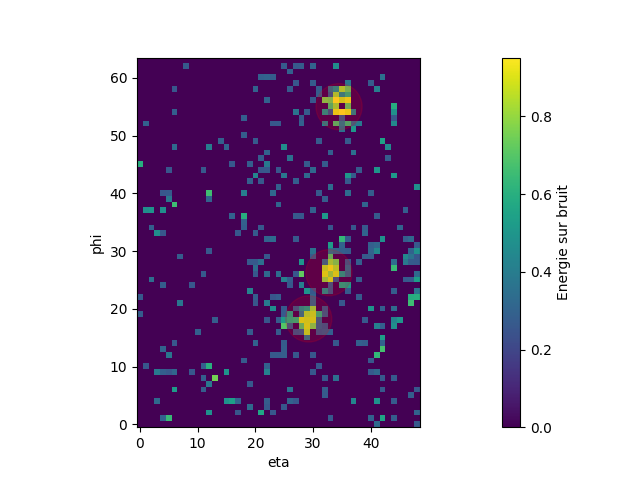
\includegraphics[scale=0.7]{Figures/dataset/matrix_post_traitement_reduced_2.png}
    \caption{Matrice d'un pas de $0.1 \times 0.1$ générée à partir de l'énergie sur bruit des cellules du calorimètre supérieure à 2 puis normalisée pour l'expérience 0 du fichier : \url{user.cantel.33075755.\_000001.calocellD3PD\_mc16\_JZW4.r14423}.}
    \label{fig:matrix_post_traitement_reduced_2}
\end{figure}

\break

\subsection{Sauvegarde des matrices}

Après toutes les étapes précédentes, nous souhaitons conserver nos matrices pour pouvoir les utiliser par la suite pour l'entraînement et l'évaluation de nos modèles.

Afin de les sauvegarder dans un format facilement utilisable et commun à de nombreux réseaux neuronaux convolutifs, nous avons décidé de multiplier toutes les valeurs de nos matrices par $255$ afin de les contenir sur $8$ bits. Grâce aux trois canaux de celles-ci, nous pouvons les représenter sous forme d'images.

Par ailleurs, il est important de n'appliquer aucune compression sur les images pour éviter de les détériorer ou d'introduire des artéfacts. Le résultat de toutes les manipulations et préparations de nos données nous donne des images semblables à la figure \ref{fig:image_type_from_dataset_49x64}.

\begin{figure}[hbt!]
    \centering
    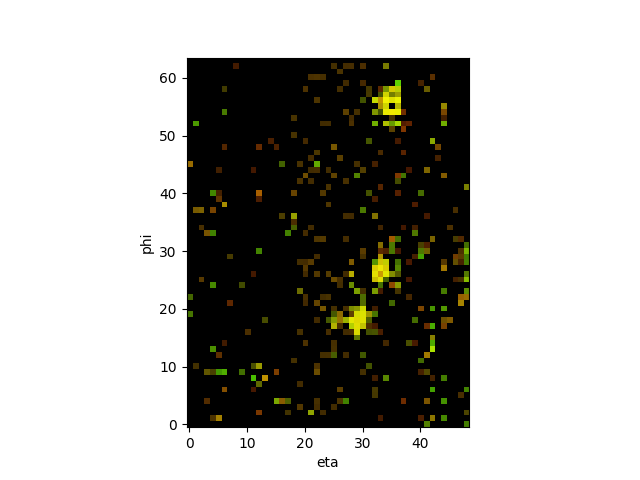
\includegraphics[scale=0.7]{Figures/dataset/image_type_from_dataset_49x64.png}
    \caption{Image construite à partir du jeu de donnée pour l'expérience 0 du fichier : \url{user.cantel.33075755.\_000001.calocellD3PD\_mc16\_JZW4.r14423}.}
    \label{fig:image_type_from_dataset_49x64}
\end{figure}

\break

Lors de ce travail, plutôt que de travailler avec des dossiers d'images, nous avons enregistré nos matrices dans des fichiers binaires .npy. Ce dernier est un format proposé par la librairie NumPy permettant d'enregistrer des tableaux facilement, et d'utiliser peu de mémoire.


\section{Manipulation et préparation des données issues des jets}

En ce qui concerne les données des jets, comme décrit dans la section \ref{sec:files_structure} nous allons utiliser les coordonnées $\eta \times \phi$ afin de calculer les indices correspondant sur nos matrices à l'aide de la même formule décrite dans la sous-section \ref{formula:compute_indices}.

Tout comme pour les données du calorimètre, nous n'utilisons que celles comprises dans l'intervalle $\eta \in \mathbb{R} : \eta \in [-2.4;2.4]$ et $\phi \in \mathbb{R} : \phi \in [-3.14;3.14]$.\\

Les données des jets sont utilisées pour générer des labels. Puisque la génération de ces derniers est différente en fonction du modèle, les explications à leur sujet sont comprises dans le chapitre traitant des modèles utilisés \ref{UsedModels}, aux sous-chapitres : \ref{subsec:yolov8_labels_generation} et \ref{subsec:resnet18+head_label_generation}.

\section{Répartition des données utilisées}

Comme indiqué initialement dans la section sur la provenance des données \ref{sec:dataset_origin}, nous possédons dix fichiers de données du calorimètre, et dix autres contenant les jets associés.

Chaque fichier contient $1000$ expériences. Ainsi, nous travaillons avec un total de $10'000$ événements. Nous avons décidé d'en sélectionner $8'000$ pour l'entraînement de nos modèles, $1'000$ sont dédiés pour la validation, et finalement les $1'000$ derniers sont utilisés comme ensemble de test. 

La sélection de ces derniers a été réalisée simplement à l'aide d'un modulo. Toutes les cinq expériences, un événement est ajouté alternativement à l'ensemble de validation ou de test.

\section{Choix des modèles de machine learning}

Initialement, notre projet devait utiliser le modèle de segmentation sémantique U-Net. En imaginant le bon fonctionnement du modèle sur les entrées, nous aurions en sortie un masque contenant les pixels appartenant aux jets, ceux correspondant aux bords des jets, ainsi que le fond.

Bien que cela soit une approche viable, en discutant plus en détail avec la professeure Anna Sfyrla de l'utilisation de la sortie du modèle, nous avons découvert les points suivants.

Outre la contrainte de vitesse, une expérience est considérée comme intéressante ou non en fonction du nombre de jets qu'elle contient et de l'énergie de ceux-ci. Il est donc pertinent d'anticiper comment la sortie va être traitée afin d'obtenir le nombre de jets et leur énergie respective. Même s'il est possible de calculer ces valeurs à partir d'un masque, il demeure plus simple et plus rapide de le faire à partir des coordonnées du centre d'un jet. Cela évite de lire chaque pixel issu du masque pour savoir s'il doit être pris en compte ou non. De plus, comme il s'agit de segmentation sémantique, nous savons uniquement si le pixel en question appartient ou non à la classe jet mais pas à quel jet, il faut donc en plus gérer cela.

C'est pour les raisons précédentes que nous utilisons des modèles de détection nous retournant le centre des jets détectés. Leur choix sera détaillé dans le chapitre qui leur est dédié (\ref{UsedModels}).

%----------------------------------------------------------------------------------------
